\documentclass{article}
\usepackage{graphicx}
\oddsidemargin 0.25in \evensidemargin 0.25in
\topmargin 0.0in
\textwidth 6.5in \textheight 9in
\headheight 0.18in \footskip 0.16in
\leftmargin -0.5in \rightmargin -0.5in

\usepackage{epsf}\usepackage{here}

\begin{document}
\noindent{\LARGE \textbf{Chebyschev Filter ($Z$-domain)}
\hspace{\fill}\textbf{Zchebyi}}\\
\normalsize
\newline
\rule{\textwidth}{0.5mm}

\noindent
Implementation of a lowpass or bandpass Chebyschev filter using a z-domain technique to enabling modeling of a high-order and/or narrow bandwidth filter.  Fixed time-step transient analysis must be used

\begin{figure}[H]
\centerline{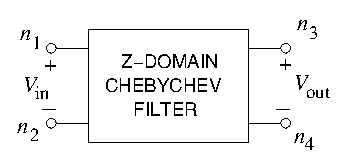
\includegraphics{figures/zchebyi.eps}}
\caption{A Chebyschev  Z-Domain filter element implemented as a voltage-controlled voltage source.}
\end{figure}

\noindent
\rule{\textwidth}{0.5mm}
\newline
\textit{Form:}
\newline
$\tt Zchebyi$:$\langle \tt{instance\ name}\rangle$ $n_1\ n_2\ n_3\ n_4\ $
$\langle \tt{parameter\ list}\rangle$
\newline
\begin{tabular}{r l}
$n_1$, $n_2\ \cdots$ & are the element nodes. \\
\end{tabular}\\[0.05in]

\noindent
\textit{Parameters:}\\[0.05in]

\noindent{\small
\begin{tabular}{|p{2.6in}|l|c|p{2.2in}|}
\hline
Parameter&Type&Default&Required?\\
\hline\hline
flp: Lower Pass Frequency (Hz) & DOUBLE& 0& reqd. if fo and pbw not specified\\
fhp: Upper Pass Frequency (Hz) & DOUBLE& 0& reqd. if fo and pbw not specified\\
fo: Center Frequency (Hz) &DOUBLE & 0 & reqd. if flp and fhp not specified\\
pbw: Passband bandwidth (Hz or \%) & DOUBLE& 0& reqd. if flp fhp are not specified\\
pbfdb: Passband Flatness (negative) (dB) & DOUBLE & $-3$ & optional\\
fls: Lower Stop Frequency (Hz)&DOUBLE& 0 & reqd. if pord not specified\\
fhs: Upper Stop Frequency (Hz)&DOUBLE& 0 & reqd. if pord not specified\\
sbadb: Stopband Attenuation (negative) (dB)&DOUBLE& $-10$ & reqd. if pord not specified\\
pord: Lowpass Prototype Filter Order& INTEGER& 0 & reqd. if fls \& fhs \& sbadb not specified\\
ildb: Insertion Loss (negative) (dB)& DOUBLE & 0 & no \\
rep: Record filter design info in report&BOOLEAN & FALSE & optional\\
\hline
\end{tabular}}\\[0.05in]

\noindent
\textit{Notes on Parameters:}\\[0.05in]
Lowpass filter is chosen if \texttt{fo} and \texttt{pbw} are not set, and  \texttt{flp} = 0. Then \texttt{fhp} is the corner frequency of the lowpass filter. Note that \texttt{fhs} must be set.\\[0.05in]
Bandpass filter is chosen by setting either ((\texttt{flp}$\ne 0$) AND \texttt{fhp}) OR (\texttt{fo} AND \texttt{pbw})\\[0.05in]


\noindent
\textit{Description:}\\
This is a v-to-v transducer implementing a unilateral Z-domain Butterworth
lowpass or bandpass discrete-time filter.  The sampling frequency
of the filter is fixed to the time-step, \texttt{tstep}, of transient
simulation. Note that this filter will not work with variable
time-stepping!  Also, the `DC gain' of the filter is 1.

The order of the filter is
determined by the netlist specifications.  Implementation of the
filter is in cascade form of conjugate pole pair blocks for even
order filters.  Odd order filters put the single real pole block
at the front of the cascade of pole pair blocks for best numerical
properties.\\[0.05in]

\noindent
\textit{Version:}
2008.01.05 \\


\begin{minipage}{\textwidth}
\rule{\textwidth}{0.5mm}
\noindent
\textit{Credits:}\\
\begin{tabular}{l l l l}
Name & Affiliation & Date & Links \\
Frank P. Hart & NC State University & Jan. 24, 2005 & \epsfxsize=1in\epsfbox{figures/logo.eps} \\
Michael B. Steer & NC State University & Jan. 5, 2008 & \epsfxsize=1in\epsfbox{figures/logo.eps} \\
 & & & www.ncsu.edu    \\
\end{tabular}
\end{minipage}
\end{document}




